\documentclass{./llncs2e/llncs}
\usepackage{graphicx}
\usepackage{fixltx2e}
\usepackage{mathtools}
\usepackage[nolist,nohyperlinks]{acronym}
% Maintain images and tables within their respective sections
\usepackage[section]{placeins}

% Scientific notation
\usepackage[scientific-notation=true, round-precision=2, round-mode=figures]{siunitx}

%
% Change the margins
%
% \usepackage[margin=2.9cm]{geometry}

\begin{document}
\title{Smart Places}

\subtitle{A framework to develop proximity-based mobile applications}
\author{Samuel Coelho, samuelfcmc@gmail.com}
\institute{Instituto Superior T\'{e}cnico}

\maketitle

% make a proper TOC despite llncs
\setcounter{tocdepth}{2}
\makeatletter
\renewcommand*\l@author[2]{}
\renewcommand*\l@title[2]{}
\makeatletter

\tableofcontents

\newpage
%!TEX root = ../report.tex

% 
% Abstract 
% 

\begin{abstract}
% Proximity-based apps are... POIs
% Increasing popularity
% Based on this the concept of Smart Place is introduced
% We have several technologies
% Bluetooth Low Energy can be used indoors
% The space owner only need to install small devices,
% BLE Beacons that broadcast an identifier
% Apps can get this identifier and offer different
% possibilities to the user according to it
% Development process implies to write the code
% for getting beacons' ids and get information
% about each POI from the backend
% One app need to be installed for each Smart Place.
% Here, we introduce a solution to make development
% of apps for smart places much easier and faster
% Developers have abstractions for the technology
% that is being used and for communication with the backend
% Also, in this solution, they write the code using
% technologies for web development, such as HTML, CSS and Javascript
% as they would do for creating any web application
% The users and owners of Smart Places just need to install
% one app. With this app, users can interact with the
% Smart Place and the owners can manage it in order to choose
% the apps that will run on their places.

Proximity-based apps engage users while they are in proximity
of Points of Interest (POIs). These apps are becoming popular
between the users of mobile devices..
Based on this, the concept of Smart Place is introduced
and is defined as a place that has some POIs that
allows users to interact with them. Several technologies can
be used.
BLE Beacons are an alternative to GPS, that does not perform well
indoors, that just require the deployment
of these small devices. They broadcast an identifier, using
Bluetooth Low Energy, that mobile
apps can get and offer different possibilities, to the users.
To develop apps for Smart Places we need
to write the code that gets the beacons' identifiers and
get more information about the POI for each identifier from
a backend. Also, users need to install one app for each Smart Place.
Here, we introduce a solution to make the development of mobile
apps for smart places much easier and faster than the existing
solutions. Also, with benefits for users and owners of
such Smart Places. Users will only need one app to interact
with any Smart Place. The same app will be used, by owners,
to configure the POIs.

\end{abstract}
%!TEX root = ../report.tex

% 
% Keywords 
% 

\begin{keywords}

proximity-based; mobile apps; smart places; bluetooth; beacons 

\end{keywords}
%!TEX root = ../report.tex

%
% Introduction
%

\section{Introduction}
\label{sec:introduction}

% General description of the problem and its context, current 
% solutions, and road map of the project.
% 2 - 3 pages
% TODO: Mobile proximity based apps (Special kind of context aware), Explain context-aware, Examples
% Technologies to know if the user is nearby some POI
% Development of proximity-based apps
% Smart spaces
% TODO: What are native and web mobile apps
% TODO: What makes more sense to proximity-based apps
% (Native vs Web)
% This paper is about...
% Present next sections

% Problem
The use of context-aware mobile apps has been increasing.
Context-aware mobile apps are apps that use data, acquired
from one or more sensors and other user's data, 
such as the calendar. For instance, it is possible to
build an app that puts the phone, in silent mode, if the
user is in a meeting. Proximity-based apps are
context-aware apps that allow the user to interact
with the app if he is nearby some point of interest.
Table \ref{tab:app_comparison} shows some statistics
about the most popular apps, in Google Play Store,
including examples of proximity-based apps,
such as Foursquare\footnote{https://foursquare.com},
Skout\footnote{http://www.skout.com/} and
Tinder\footnote{http://www.gotinder.com/}

\begin{table}[h]
\centering
\begin{tabular}{|c|r|r|}
\hline
\textbf{App} & \multicolumn{1}{c|}{\textbf{Nr of Downloads}} & \multicolumn{1}{c|}{\textbf{User Rating (0 to 5)}} \\ \hline
Facebook & 1-\num{5e9} & 4.0 \\ \hline
Twitter & 1-\num{5e8} & 4.1 \\ \hline
Instagram & 1-\num{5e8} & 4.5 \\ \hline
Foursquare & 1-\num{5e7} & 4.1 \\ \hline
Skout & 1-\num{5e7} & 4.1 \\ \hline
Tinder & 1-\num{5e7} & 4.1 \\ \hline
\end{tabular}
\caption{Some statistics about most used apps including some
proximity-based ones in Google Play Store. 
Source: App Annie (http://www.appannie.com/) 
in 2, December, 2014}
\label{tab:app_comparison}
\end{table}

Facebook is the app with the
greatest number of downloads. One of the 
proximity-based apps has, at least, \num{1e7} downloads.
Facebook has, at least, \num{1e9}. Twitter and Instagram
have, at least, \num{1e8} downloads. Which means, one of
the proximity-based apps represents
1/100 of Facebook's downloads and 1/10 of Twitter's
and Instagram's downloads. In terms of rating, all apps
have similar values

% Possible solutions
To know if the user is nearby some point of interest,
we need to know the user's location. We can use GPS to
get this information. Most apps use this technology because
most smartphones have a GPS receiver. 
%Show some statistics about smartphones with GPS
Unfortunately, GPS cannot be used indoors. The signal can
be very weak inside a building. To make proximity-based
apps work properly indoors, we need to use other 
technologies.
\subsection{Bluetooth Low Energy}
\label{sub:bluetooth_low_energy}
Bluetooth is a wireless short-range communication technology.
Bluetooth Low Energy (BLE)\cite{martellibluetooth} 
is an improvement of classic Bluetooth since it consumes 
very low power.
And that is the main reason for this technology to start to 
be used for proximity-based mobile apps,

BLE Beacons are devices, that use BLE, to broadcast a 
universally unique identifier (UUID). 
These devices use iBeacon protocol, which was created
by Apple\texttrademark. In this protocol the beacons
advertise the following sets of bytes:
\begin{description}
  \item[UUID] has 16 bytes and it's used to differentiate a 
  large group of related beacons
  \item[Major] has 2 bytes and it's used to distinguish a smaller 
  subset of beacons within the larger group
  \item[Minor] has 2 bytes and it's used to distinguish individual
  beacons within the smaller subset
\end{description}
A smartphone that
has BLE can get this signal with the mentioned bytes.
But, only smartphones
with Bluetooth, at least, version 4, have BLE.
For instance, a store owner wants to advertise a promotion
to potential customers that are nearby his store. To 
achieve this goal, the store owner would need to put
a beacon inside his store and his customers would need an
app that would get the beacon's signal and show a 
notification in the customers' smartphones,
as it is shown figure \ref{fig:store_example}.
\begin{figure}[!ht]
  \centering
    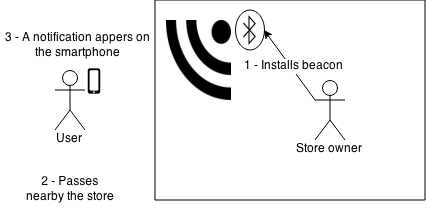
\includegraphics[width=0.9\textwidth]{img/store_example}
    \caption{Interaction between the user's smartphone
    and a beacon inside a store}
    \label{fig:store_example}
\end{figure}

To develop these apps, that use beacons, we can use the 
BLE API that each 
mobile platform provides or simply the Software
Development Kit (SDK) from the 
beacons vendor. The example of the store owner is a
simple one. The app just gets the signal and show a 
notification. However, if the store owner has more than
one store and wants to show a different promotion depending
on each store, the app would need to do more than just get
the beacon's signal. After getting the signal, the app
would get the promotion for that beacon, from a 
backend. The developer of this app, would need to
write the code that gets the beacon's signal and also
the code that will get the information from the backend.

Another example could be an app for a museum. The owner
of a museum wants to show more information, in the 
visitors' smartphones, about the pieces that are in a given
room. He would need one beacon for each piece and an app
that would get the beacon's signal and use a
backend to get the right information about a given piece.
The museum needs to advertise, to its visitors, that such
an app exists and also, tell them to download the app
before they enter the museum. The developers of the
store and the museum apps will write similar code to get
the beacon's signal and get data from a backend.

\subsection{Smart Places}
\label{sub:smart_places}
Before going further, we will introduce the concept of
Smart Place. Smart places are places that can, somehow,
interact with users nearby and users can interact 
with them.
In this context, a smart place have beacons and the users
have apps, installed in their smartphones, that can interact
with them and show relevant information to the user.
With this definition, we can say, for instance
that the owner of the store, wants to
turn his store into a Smart Place.
The same applies to the museum owner.
The user would need to install two apps, one for the
store and another one for the museum.
If there is another Smart Place, the user would need to
install another app.

Any mobile app can be a native or a web app. Native apps
are apps that we have to install and that can access
device's features, such as BLE. Web apps are web
applications, designed for mobile devices, that run
on the device's browser. Table \ref{tab:native_vs_web}
compares some characteristics of both kinds of apps.
% Table Native vs web
\begin{table}[h]
\centering
\begin{tabular}{|c|c|c|l}
\cline{1-3}
 & Native & Web &  \\ \cline{1-3}
\begin{tabular}[c]{@{}c@{}}Access to device's features \\ (Camera, accelerometer,etc)\end{tabular} & All & Limited &  \\ \cline{1-3}
Installation needs & \begin{tabular}[c]{@{}c@{}}Need to install\\ the app\end{tabular} & \begin{tabular}[c]{@{}c@{}}Only a web browser\\ is needed\end{tabular} &  \\ \cline{1-3}
\begin{tabular}[c]{@{}c@{}}Method for finding\\ the app\end{tabular} & App stores & \begin{tabular}[c]{@{}c@{}}Users have to find\\ it somewhere\end{tabular} &  \\ \hline
Updates & \begin{tabular}[c]{@{}c@{}}Users can choose\\ to not update the\\ app\end{tabular} & \begin{tabular}[c]{@{}c@{}}All users have\\ access to the same\\ version\end{tabular} &  \\ \cline{1-3}
Where it can run & \begin{tabular}[c]{@{}c@{}}Only on the platform\\ for which it was\\ developed for\end{tabular} & On any platform &  \\ \cline{1-3}
\end{tabular}
\caption{A comparison of some characteristics of Native and Web mobile apps}
\label{tab:native_vs_web}
\end{table}
This apps do not need to be
installed but they do not have access
to same device's features that native apps have.
Mobile apps for smart spaces, according to our definition,
need to be native, because we need to get signals from
nearby beacons. For that, we need to use bluetooth, which is
not available in web apps, since they run in the browser.
A solution to allow developers to get the best of both sides
is proposed here. In one side,
native apps can detect nearby beacons. In the other side,
web apps do not need to be installed.

In next section \ref{sec:objectives}, we describe the main
objectives of the project proposed here.
Section \ref{sec:related_work} describes related
work about the development and deployment of
context aware mobile apps.
In \ref{sec:architecture} it is explained the architecture of our solution. The main components and the role of
each one.
Section \ref{sec:evaluation} is about how we are going
to evaluate our solution.
Finally, last section \ref{sec:conclusions} we summarize
the main ideas of the entire document.

%!TEX root = ../report.tex

% 
% Objectives
% 

\section{Objectives}
\label{sec:objectives}
% ~1 page
%Clearly explain the project objectives.

% Develop a framework that allows...
% Develop an app for a smart place, abstracting
% beacons, think only in POI and their meaning
% Users only need one app for any smart place
% The same app can be used, for space owners, to install apps
As was mentioned in section \ref{sec:introduction} we purposed
to develop a framework to develop proximity-based web mobile
apps, or, according to our definition of smart place, web
mobile apps for smart places.
Part of the framework will need to run in the user's 
mobile device.
Given that, we have two main objectives. First, the framework
itself and second, the Smart Places App.

The framework should allow developers to develop their apps,
without needing to write the code to get the beacons' signals
and get more information from the back-end. That would be the
framework's job. Developers would only need to write the code
that will run in each POI. Each POI would have a name and
some parameters specified by the developer. 
For instance, in the example of the restaurant,
in \ref{sec:introduction}, the POI could have the name Table and
a parameter could be the number of the table.
Developers would only need to write their apps using web
technologies, such as HTML and JavaScript.

Part of the framework will run on the users' smartphones.
We will develop the Smart Places App, for Android, which would
be an  app that will scan for beacons, and will get the 
corresponding information about the POIs that are being 
represented by the scanned beacons.
The user will be notified about the POIs
that were found and then, he can select one of them and
start using the associated app. 
Also, the smart place owner, would be able to use this app
to install apps, developed using this framework, in his
smart place.

To summarize, the framework will allow developers to develop
apps for smart places using nothing more than web technologies
and without writing the code to scan nearby beacons.
The Smart Places App will allow the users to access any app,
developed using this framework, in any smart place. Also,
the smart places owner could install apps in their spaces
using this same app.

%!TEX root = ../report.tex

%
% Related work
%

\section{Related Work}
\label{sec:related_work}
In this section we discuss some related work.
For each one we describe its limitations and its main
benefits, providing, at the same time, motivation
to develop our framework.

\subsection{BLE Beacons applications}
\label{sub:ble_beacons_applications}
% Why
% For each one: What, Pros, Cons
BLE Beacons are going to
be used to develop proximity-based apps
on top of it. Some
applications, where this technology is used,
will be presented here, to
get good insight about the potential use cases of this 
technology and the apps developed using it.
\\
% BlueSentinel
\textbf{BlueSentinel\cite{Conte2014}:} is a 
occupancy detection system, for smart buildings,
that uses BLE Beacons to detect the presence of
people. The concept of a smart building
is similar to Smart Place,
due to the existence of sensors and actuators.
It is focused on the power efficiency of the
building. The idea is to optimize energy
consumption according to people's presence.
For instance, if there are no people in a given room,
the heating system can be turned off.
In this solution, the users have to install
an app, that will get the beacons' signal and
send data to a server, which will process it
and send requests to actuators in order to
perform actions to optimize the
building's power efficiency.
Unfortunately, there is a limitation
of iBeacon protocol implementation
in iOS. Beacons can be received, by the apps,
only when these are active. When the apps are in
background, they are waken up only to handle
enter/exit region events. To circumvent this
limitation, the authors developed custom
beacons, which advertise more than one region
in a cyclic sequence. These custom beacons
were created using an 
Arduino\footnote{http://www.arduino.cc/}
and an Bluetooth USB BLE dongle.
Since this solution is a native app,
users have to install it in order
to make the smart building work to
optimize power efficiency.
Once the user starts the app, he does not
need to interact with it anymore, since it
will run in background.
\\
% Blue View
\textbf{BlueView\cite{Chen2013}:} is a system to help
visually impaired people to perceive some POIs.
This solution has two main components: The viewer device
and the Beacon Points (BPs). The first one is a mobile phone,
carried by the user, which is bluetooth-enabled.
The Beacon Points are just bluetooth tags instead of
BLE Beacons. The name of a POI is associated with
MAC address of the tag which it is associated to.
The steps involved in using the system are the
following: first, the viewer device will scan
for nearby BPs; then, a list of the names of
BPs is created. This list is refreshed anytime a new
BP is detected and the user is informed through auditory
feedback. The second step consists of the user, using
the viewer device, establishing a connection with a BP
attached to an object. Finally, using audio prompt, the BP
will assist the user in locating the object.
Despite of this solution being a mobile app, installed
in the viewer device, the authors do not have in
consideration the typical concerns of any mobile app,
such as the energy consumption.
The authors tested the application, in 2013,
using Nokia N70 as the viewer device.
This solution could be implemented using BLE Beacons
and the viewer device could be any Android, iOS or
Windows Phone smartphone.
For the audio features the smartphone's speaker or
a custom BLE Beacon with a built-in speaker could be
used.
\\
% MOSES
\textbf{MOSES
(Mobile Opportunistic System for Experience Sharing)\cite{BenAbdesslem2014}:}
% In exhibitions, share experiences and communicate with
% other participants
% Roaming charges... No Internet access
% They have smartphones with comm techs like bluetooth and wifi
% Share experience (text or multimedia content)
% Shared content is geo-tagged
% Available to participants in the same location
% Or will be visiting the area later on
% Using DTN
% When content is created is shared with other users
% in range in an epidemic fashion
% Each user share his content and content
% received by other users
% Implemented in Android
% Geo-tagging:
% -> GPS, WiFi, cellular positioning
% -> Indoor, estimote beacons
% -> Equipment: Smartphones, Beacons, Raspberry Pies
% Raspberry pie: Collect all content created by participants
% and emulate an intermittent internet connection
% Act as a WiFi access point
is a solution to allow
participants of exhibitions, to share experiences and
communicate with other participants.
The participants can share their experiences using
just text or they can add multimedia content.
This shared content is geo-tagged, which means that
it will be available to other participants in the same
location.
Most of these events are international. 
Due to the
roaming charges most users will not have an
Internet connection available in their mobile devices.
However, most of the participants have smartphones
equipped with communication technologies such as
Bluetooth and WiFi.
To circumvent this limitation, this solution
uses a Delay Tolerant Network (DTN)\cite{pateldelay}.
When content is created it is shared with other
users in range. Each user shares the created content and the content received by other users.
This solution was implemented in Android.
Geo-tagging is performed using usual positioning
systems, such as GPS, WiFi and cellular positioning.
For indoor positioning it uses 
Estimote\footnote{http://estimote.com/} beacons.
Besides the smartphones and the beacons, this
solution also uses a 
Raspberry Pi\footnote{http://www.raspberrypi.org/}.
This device is used to collect all content created by
participants and it emulates an intermittent Internet
connection, acting as a WiFi access point.
\\
% Context capture
\textbf{ContextCapture\cite{Antila2011}:}
% Usage of context-based awareness in status updates
% Allows users to add different descriptions of context 
% information to their Twitter messages
% and Facebook status updates in a narrative format
% Indoor location: BLE Beacons
% Two main goals:
% Demonstrates technical aspects of collaborative
% context
% Test and analyze the UX of context-aware systems
% Include contextual information to status updates
% in Facebook and Twitter 
% User can decide the abstraction level
% (Coordinates, address or semantic label
% such as "conference venue")
% Mobile app and server-side integrated with Facebook and 
% Twitter
% Mobile app gathers context from device itself,
% sensors and from nearby devices using Bluetooth
% Format: “[User-defined message] Sent
% from [Location] while [Activity]
% [Description] [Topic] and [Applications Activity] with 
% [Friends].”
In this work, the authors try to use
context-based information to allow users to
add more information to their status updates
in the main social networks, such as
Facebook\footnote{http://www.facebook.com} and 
Twitter\footnote{http://twitter.com}.
This work had two main goals: first, demonstrate technical
aspects of collaborative context, such as,
how to get contextual information from
surrounding devices and how they can be used
as a source of contextual information;
second, test and analyze the user experience of
context-aware systems.
The user can decide the abstraction level (coordinates,
address or semantic label).
The authors implemented a mobile app and a
server integrated with Facebook and Twitter.
Context information comes from the smartphone itself,
from its sensors and from the nearby devices through
Bluetooth. 
Devices can be other smartphones or BLE Beacons, which
are used for indoor location.
Similarly to \cite{BenAbdesslem2014}, devices communicate
with each other as a network.
Using this solution, the user can create status updates,
in the mentioned social networks, in the following format:
\\
``
[User-defined message] 

Sent from [Location] while [Activity]

[Description] [Topic] and [Applications Activity] with 
[Friends].
''
\\
\subsection{Frameworks to develop and deploy 
context-aware mobile apps}
\label{sub:frameworks_context_aware}
In this section we describe related work about the
development and deployment of mobile native and web 
context-aware applications.
Since we propose a framework to develop
proximity-based apps, the state
of the art of existing frameworks, that deliver
context information to the apps will be presented.
\\
% DTN
\textbf{Dynamic frameworks for 
mobile web DTN applications:}
There are multiple frameworks to deploy localized
mobile native or web apps, even if the user is using an
unstable Internet connection. One example of this
kind of framework is the one
described in Sankaran et al.\cite{Sankaran2014}.
This framework supports the deployment of localized 
native and
web apps in Delay Tolerant Networks (DTNs).
A DTN is a computer network that 
addresses issues about the lack of continuous network
connectivity. 
Mobile networks are good examples of DTNs,
because, most of the times, the connection is not stable.
Usually, the user is moving, along with his mobile 
device.
It is expected that the connection sometimes is not
available.  
This solution also has an embedded web server 
and has an implementation that runs on a PC, which allow
developers to test their applications before deploying
to production environment.
However, the owner of a given point of interest does not
have access to any interface to install apps that will
belong to that point. Also, it does not support, in the
same app, multiple points of interest with different
meanings and different behavior in each one of them.
\\
% Framework for Developing Distributed Location Based 
% Applications
\textbf{Frameworks for developing distributed
location-based applications}
% Develop location based apps
% Discuss several technologies for positioning
% GPS, GSM, WiFi and Bluetooth
% Advantages and disadvantages of each one
% Architecture
% -> GPS receiver, bluetooth receiver, WiFi receiver
% -> Mobile device
% -> Database Server, Application server
% Application server provides web services for
% mobile clients and communicates with the
% database server
% Client communication (SOAP message)
% Querying the database (native communication)
% Mobile device get geographical coordinates from
% several devices;
% Send this data, in a SOAP message, to the
% appropriate web service in the Application Server
% App server communicates with Database server
% to query the database
% Database server sends a response back with
% location information if there is any, for that
% particular group of coordinates
% No evaluation
% Location info can come from any source
% Only for native apps (No web apps)
% Does not take into account constraints in terms
% of resources, such as lack of internet connection
% and battery
% SOAP could be replaced by REST [PAPER]
In the work presented in Krevl et al.\cite{Krevl2006}, 
a framework
was developed to allow developers to build
location-based apps. Location information can come
from any source, such as GPS receivers, Bluetooth
receivers and WiFi receivers.
The authors discuss some benefits and limitations
of several technologies for getting the
user's positioning.
In terms of architecture, the main components
are:
\begin{itemize}
\item
Devices that are used to get location data, such as
the ones already mentioned. 
\item The users' mobile devices.
\item The Database Server, which is where the mapping
between geographical coordinates and location
information is stored.
\item And, the Application Server, which provides web services for
mobile clients. This server also communicates
with the Database Server.
\end{itemize}
The mobile device get geographical coordinates
from any source and send that data, in a
SOAP \cite{Seely:2001:SCP:560836} message,
to the appropriate web service in the Application
Server. This server, communicates with the Database Server
to query the database, which sends back a response with
location information, if there is any, for that
particular group of geographical coordinates.
The authors did not evaluate the system.

In this solution, geographical coordinates can
come from any source. It is a good approach for
mobile native apps, but, it does not support web apps.
The authors do not take into consideration
constraints in terms of resources, such as
lack of Internet connection and battery.
Since most users have limited data plans for
their smartphones and SOAP messages can
grow, in size, due to its XML format,
RESTful \cite{richardson2008restful}
web services could be used instead
\footnote{Work about migrating from SOAP web services
to RESTful in \cite{upadhyaya2011migration}}.
\\
% Dynamix
\textbf{Dynamix\cite{Carlson2012}:}
is a framework to develop
mobile native and web apps that allow them to receive
context information, for instance, position and device's
orientation. This framework has plug-ins that get
one or more sensor's raw data and turn that into event
objects, that contain more high-level information.
This framework supports many kinds of context information
and it is possible to develop more plug-ins to allow the
apps to generate additional events that are not
already supported. It is similar to the previous
framework but is more focused on delivering context
information to apps instead of deploying them.

To achieve our goal, our framework could be just a
plug-in for Dynamix. The plug-in would
need to get the beacon's raw data and
turn that into a more high-level information 
using a backend. In this framework,
the user needs to install an app, that manages the service
that runs in background, and needs to define some
security policies. This could mean a big overhead since
we are more focused on developing proximity-based
web applications, that do not require such complex security
policies because, in this kind of apps, there is only need
to access the device's sensors that could provide,
to the applications, positioning data. 
In our framework, the user would only need to
install one app, let it run in background and turn on
bluetooth. Also, this does not offer a complete solution
since the owner of one or more points of interest
has no way of installing new apps on them.

\subsection{APIs and Frameworks to develop mobile native apps 
using HTML, CSS and Javascript}
\label{sub:frameworks_web}
Since we propose a framework to develop proximity-based
mobile web apps, a good insight, about some existing
solutions to develop mobile apps using web technologies,
such as HTML, CSS and Javascript, is needed.
These solutions, described below, allow developers to
write their apps, using HTML, CSS and Javascript, as
if they are web apps and deploy them in most used app
stores, such as 
Google Play\footnote{https://play.google.com/}
and
App Store \footnote{http://store.apple.com/}.
\\
\textbf{Cordova:}\footnote{http://cordova.apache.org/}
is a set of APIs that allow developers to access
devices' functionalities, such as the camera or
accelerometer, from Javascript code.
To access such functionalities developers build plugins.
Any developer can develop plugins and use plugins
developed by others.
\\
%Phonegap
\textbf{PhoneGap}:\footnote{http://phonegap.com/}
is a framework to develop mobile apps
using web technologies, such as HTML and JavaScript. The
same code is deployed, as a native app, to multiple mobile
platforms. Each app is nothing more than an embedded browser
that runs a local web application. 
Using some plugins from Cordova, the apps can access some
device's functionalities, such as bluetooth. 
However, to develop proximity-based apps, such as
the ones mentioned in 
\ref{sub:ble_beacons_applications},
the developer has to configure a backend and write the
code that will interact with it. Also, since the apps are
installed as native ones, the user needs to install
an app for each place where each app works.
\\
%Ionic
\textbf{Ionic:}\footnote{http://ionicframework.com/}
is a framework very similar to PhoneGap. When using
this framework, developers are allowed to use Cordova
plugins, similarly to PhoneGap. It includes a
Command-Line Interface to initialize the structure
of a new app. Also, a new app already includes Javascript
files that use 
AngularJS\footnote{https://angularjs.org/}, 
which is a framework, for frontend development,
to build web pages with dynamic content.
However, it has the same benefits and limitations
than PhoneGap.

\subsection{Summary}
\label{sub:summary}
To finish this section, each related work has its own
advantages and limitations.
In \ref{sub:ble_beacons_applications} some
examples of proximity-based apps were described.
In \ref{sub:frameworks_context_aware} there is
some discussion about some
frameworks for developing context-aware mobile apps,
including their limitations.
Most of them, only support mobile native apps and
do not offer a complete solution, since the developer,
needs to configure a backend and write the code that
receive the beacons' signals and sends data retrieved by 
the beacons to the backend, in order to build 
proximity-based apps using BLE Beacons.
Finally, in \ref{sub:frameworks_web}, there are
examples of frameworks for developing mobile apps
using HTML, CSS and Javascript, allowing developers
to write the code as they are creating web applications
and deploy them in the app store of more than one
mobile Operating System.
In terms of development of proximity-based apps,
these solutions have the same disadvantages of the
ones in \ref{sub:frameworks_context_aware}.
None of those solutions offer abstractions to
the technology used to get information about POIs.
Our framework, described in the next section, tries 
to offer a complete solution that solves all
these limitations, in such a way that, developers do not
need to think about the technology behind proximity-based
apps, but only about the application logic and the meaning
of each point of interest.
%!TEX root = ../report.tex

% 
% Architecture
% 

% 2/3 pages
%Your proposed architecture. Can have lots of pictures and 
% bullet points so it is easy to understand.
\section{Architecture}
\label{sec:architecture}
We propose a framework to develop mobile web apps for smart
places, that allow developers to only write the code
for the application logic and the specific behavior when
the user is nearby specific points of interest (POI).
Each beacon represents one POI. Developers will not need
to write the code that gets beacons' data and get the
right information from a backend. They will need only
to write the code for each specific POI. They could give
a name to each POI and the app will receive that name 
instead of the beacon's raw data. 

One of the main goals of this project is to allow
users to interact with any Smart Place, without
the need to install one native app for each one.
Mobile web apps do not need to be installed because
they run in the device's browser.
This is the main reason why our framework will
target mobile web apps instead of native ones.
This means that, when the user starts to interact
with a Smart Place, he will interact with a mobile
web app, running in his mobile device's browser.

However, detecting
nearby beacons is not a feature integrated in the mobile
Operating System. Our solution would be to build the
Smart Places App,
that detects nearby beacons, turn them into names and
other high-level information, and deliver it to the
mobile web app. The user would need only this app to
be able to access any smart place app. Also, the same app
could be used to configure a smart place.
Considering the restaurant example, mentioned in
\ref{sub:bluetooth_low_energy}, some
developers, could develop the app for restaurants,
using our framework. These developers would only think
about tables instead of beacons. The owner would need
to put a beacon in each table. After the beacons
installation, he could just use the Smart Places App,
choose the app for restaurants, and put his smartphone
closer to a beacon and configure it. This configuration
would be, for each beacon, what is the number of the table
where it is deployed. Then, his customers would only
need the Smart Places App, turn on bluetooth and they will
be notified that they can make their orders from their
smartphones.

%Solution overview
Our solution has three main components,
the BLE Beacons, as it is shown in Figure 
\ref{fig:overview_architecture}, 
the Backend and an Android app
that will run on the users' smartphones.
\begin{figure}[!ht]
  \centering
    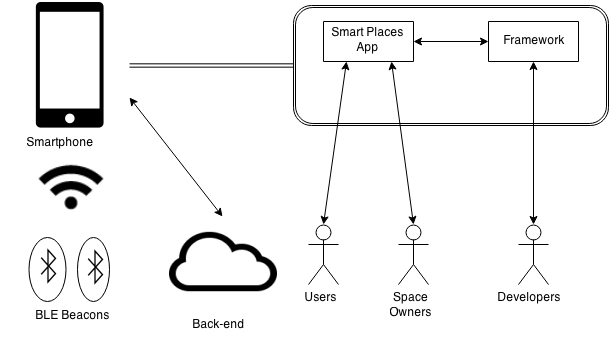
\includegraphics[width=0.9\textwidth]{img/overview_architecture}
    \caption{Overview of the proposed solution}
    \label{fig:overview_architecture}
\end{figure}
The \textbf{BLE Beacons}, as explained in section 
\ref{sec:introduction}, are small devices that broadcast
an ID using Bluetooth Low Energy. The \textbf{Backend} is where information about each beacon is stored. 
And, the users'
\textbf{smartphones}, is where the 
\textbf{Smart Places App} will run.
It is a native Android app that will scan for 
nearby beacons,
get the information about them from the Backend and
provide that information to the app associated to a 
given Smart Place.
\textbf{Users} will use this app to have access
to any app running in any Smart Place.
Also, \textbf{Smart Places Owners} can use it to configure
their Smart Places and configure which applications
will run there.
Since these apps will be mobile web apps, they will run
in a embedded browser inside the Smart Places App.
\textbf{Developers} will need to use the \textbf{Framework} to
develop such apps. Also, the Framework will provide an
Interface between the mobile web app, that will run
in a given Smart Place, and the Smart Places App.

\subsection{Smart Places App}
\label{sub:smart_places_app}
Figure \ref{fig:architecture} shows the two main
blocks that will run inside the smartphone.
We have the Smart Places App and the Framework itself.
\begin{figure}[!ht]
  \centering
    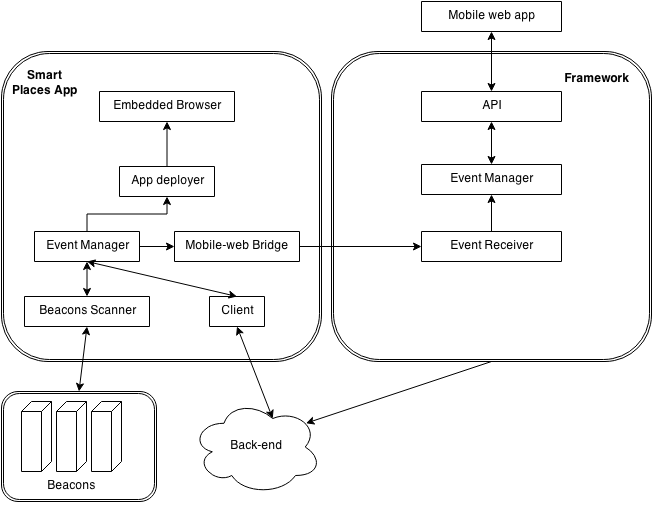
\includegraphics[width=0.9\textwidth]{img/architecture}
    \caption{Architecture}
    \label{fig:architecture}
\end{figure}
As already mentioned, the Smart Places App will be a native
Android app that the user and the Owner 
will use,
in order to be able to use any app of any Smart Place
and configure a Smart Place, respectively.
The \textbf{Beacons Scanner} will scan for nearby
beacons. After scanning, it will deliver the IDs
of the beacons to the \textbf{Beacons Manager}.
The Beacons Manager will call the \textbf{Client} to
get the information about each POI that is being
represented by each beacon from the backend or
from the \textbf{Beacons Cache}. It will be possible to
configure the Smart Places App to use the cache or not.
This cache will be an optimization to avoid communication
with the backend in each scan. If this cache is being
used, when a scan is completed, the Client will
check if the information about that beacon is in
the cache. If it is, the Client does not need to request
data from the backend. Otherwise, the Client will
request the information about all the POIs of that
Smart Place. In the next beacons scan, if we stay in
the same Smart Place, there is no need to make requests
to the backend since all the mapping between beacons
and POIs is in the cache.
After getting the POI information from the Client,
the Beacons Manager will call the \textbf{Mobile-web Bridge},
which provides an interface between the native app
and the web app, that will deliver this information
to the mobile web app that is running in the
\textbf{Embedded Browser}. 
Each time the web app needs to interact
with the native app, this component is called.
The \textbf{User Manager} is called to login the
user and to get the information about the user. 
To perform the user's login, the User Manager
will call the Client that will send the needed information
to the backend to login the user. After this step,
the mobile web app, can use the Mobile-web bridge
to get information about the logged in user.
The \textbf{Notification Service} is called to
show notifications in the user's mobile device.

\subsection{Framework}
\label{sub:framework}
The Framework provides, to developers, an \textbf{API} that they
can use to perform operations about the POIs or about the users.
Developers are allowed to define callbacks for each POI or to
even create new POIs. In order to do this, the API
uses the \textbf{POIs Manager} that will store the callbacks
for each POI.

In order to understand how the presented components
interact with each other and how the whole solution will
work, we need to take into consideration the data model
shown in Figure \ref{fig:uml}.
As mentioned in \ref{sec:introduction}, a Smart Place
is a set of POIs. Each BLE Beacon represents a POI.
Each POI has a name and a set of parameters, which are
pairs with a key and a value.
For instance, in the example of the restaurant,
introduced in section \ref{sub:bluetooth_low_energy},
each POI could have the name ``table'' and one 
parameter with key ``number'' and the value would
be the number of the table. Since the applications
that will belong to a Smart Place will be
mobile web apps, they will run in some web
server. This is why each Smart Place has an URL,
that will act as an entry point.

\begin{figure}[!ht]
  \centering
    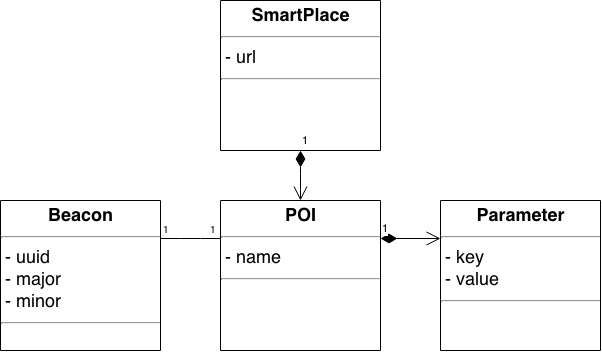
\includegraphics[width=0.9\textwidth]{img/smart-places-uml}
    \caption{Data Model}
    \label{fig:uml}
\end{figure}

% Two phases: Finding Smart Places and finding POIs
% First phase: how it works
% Second phase: how it works
% why two phases (this is not a CMS for beacons...
% more powerful...)
% Developers will only deal with POIs...

The mobile app that will be developed, 
the Smart Places App, will run in background,
scanning for nearby beacons. After the scan process,
if there are beacons that were found each one
can be mapped to one of the following kinds of
objects: Smart Place or POI.
Two phases can be considered: Finding Smart Places
and finding POIs.
As mentioned before, a Smart Place is a set of
POIs. Considering these two phases, the mobile app
will work as follows:

\begin{itemize}
\item After beacons are found, the app will try to map
these beacons to Smart Places. Figure
\ref{fig:sequence-smart-places} shows how the components
of the solution interact with each other to get
available Smart Places from the beacons that were found.
The Beacons Manager sends the list of found beacons
to the Client which will request, to the Backend,
to map those beacons to Smart Places.
After this step, the Beacons Manager calls the
Notification Service in order to show a notification
about the Smart Places that were found.
Then, the user can ignore the notification or
choose one Smart Place. If he selects one,
the Beacons Manager calls the Mobile-Web Bridge,
which will request the Embedded Browser to load
the URL of the selected Smart Place. Now, the user
will have access to the web application associated
with the Smart Place;
\item In the same Smart Place, the user will
pass near multiple POIs. The process of mapping
beacons to POIs is shown in Figure
\ref{fig:sequence-poi}.
After the previous
phase, the app will keep running in background
scanning for beacons. However, after beacons
are found, the Beacons Manager will select the
nearest beacon, that belongs to the Smart Place
that the user selected. Then, the Beacons
Manager calls the Client that will request
the Backend to get the POI object for that
beacon. After the Client receives the response,
it is sent back to the Beacons Manager, which will
call the Notification Service to show a notification,
in the user's mobile device, about the POI that was
found. After the user clicks on the notification,
the Beacons Manager will call the Mobile-Web
Bridge to deliver the POI object to the mobile
web application that belongs to the Smart Place
and is running in the Embedded Browser.
\end{itemize}

\begin{figure}[!ht]
  \centering
    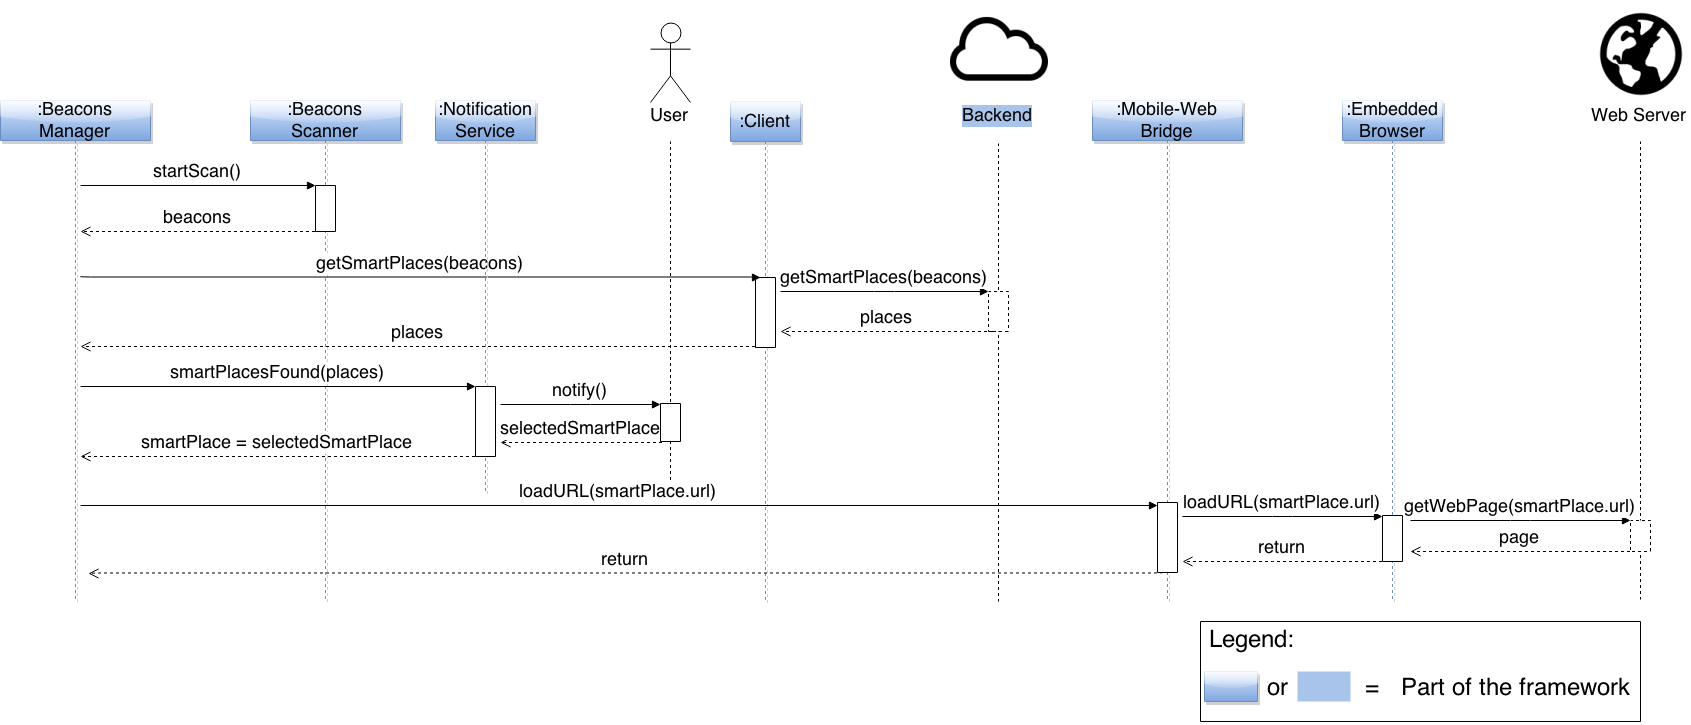
\includegraphics[width=1\textwidth]{img/smart-places-sequence}
    \caption{Sequence Diagram}
    \label{fig:sequence-smart-places}
\end{figure}

\begin{figure}[!ht]
  \centering
    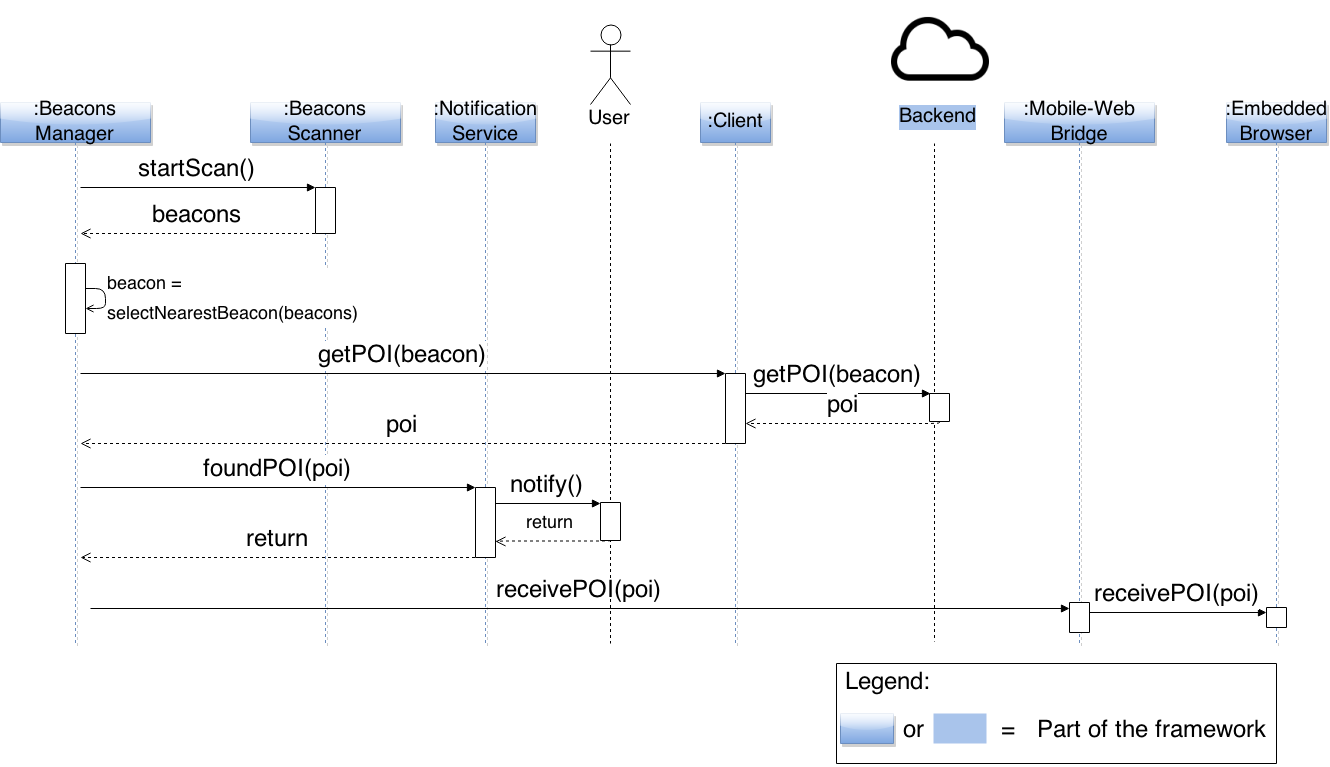
\includegraphics[width=1\textwidth]{img/smart-places-poi-sequence}
    \caption{Sequence Diagram}
    \label{fig:sequence-poi}
\end{figure}

As mentioned before, all the mapping between
beacons and Smart Places and POIs will be handled
by the framework. Developers will be able
to develop their applications without having to
configure any backend and writing code to handle
the BLE Beacons.
They will only write the code
that will run inside the Embedded Browser.
Their applications will receive POI objects,
which can be handled by any function. Since
these functions will run in the mobile
device's browser sandbox there are no security
issues about any malicious code.

In terms of development of the framework there are
several technical challenges:
\begin{itemize}

\item The time interval, between each
scan process.
If this value is too high
some beacons can be missed and the user will
not be able to interact with some Smart Places.
If this value is too low, the user will run out
of battery faster than usual;

\item If the user is nearby a lot of Smart Places
too many notifications can appear in his mobile
device. A solution could be to put all
the Smart Places that were found in just one
notification. However, when the user moves more
beacons can be scanned and more Smart Places
will be discovered and the user will receive
more notifications;

\item Get the nearest beacon. As explained before,
when the user chose a Smart Place, the mobile
app will keep on running in background 
trying to map beacons to POIs. Only the
nearest beacon is selected in each scan.
Most beacons vendors provide SDKs to handle
scanning and getting information from the beacons.
Most of them allow developers to get the distance.
Unfortunately, the method used to get this
value is not so accurate because it relies on the strength
of the signal, which can be very weak due to
many factors besides the distance, since it
is a wireless signal.

\item How to pass POI objects from the mobile
app to the web application running inside the
Embedded Browser.
The application that belong to a Smart Place
will run in the mobile device's browser.
However, after mapping beacons to POI objects,
those objects need to be passed to the 
application in the browser. This objects
are acquired by the mobile app that runs
native code and need to be passed to
code that is running in the browser
that is typically Javascript and not native.

\end{itemize}

In section \ref{sub:summary} the main limitations 
of related work were presented.
The solution being proposed here tries to
circumvent them. The Smart Places App will
offer, to the owners of Smart Places, an interface
where they can manage their POIs.
In terms of communication with the backend,
REST\cite{richardson2008restful} will be used instead
of SOAP. To invoke SOAP web services the client needs
to get the specification from a 
WSDL\footnote{Web Services Description Language:
http://www.w3.org/TR/wsdl} file, specify the
transport protocol and encode the request in a
XML\footnote{Extensible Markup Language:
http://www.w3.org/XML/} document. To invoke a
RESTful web service the client just needs to know
the endpoints and make an 
HTTP\footnote{Hypertext Transfer Protocol:
http://tools.ietf.org/html/rfc7235} request.
If messages are encoding in 
JSON\footnote{JavaScript Object Notation:
http://www.json.org/}, they will
get smaller than if they were encoded in XML.
This is important to consider in a resource constrained
mobile environment. SOAP is more flexible than REST
because any transport protocol can be used and it is
possible to add headers to handle security features.
However, we do not need such flexibility.
Another limitation of related work is that developers
have to write code to interact with the technology
where location data comes from. Our solution aims to
create abstractions for the BLE Beacons, which is the
technology being used to get location data.
Our mobile app will scan for beacons and get all the
needed data from the backend. Developers will only have
to use POI objects instead of identifiers of beacons.
The mapping between beacons and POIs will be performed
by the framework.
In terms of permissions, our app will only need the
user to turn on the Bluetooth receiver of his
mobile device. He will not have to configure
anything else in order to use it.
To avoid to make the user install one native app
in order to be able to interact with a Smart Place
our solution will allow developers to develop their
applications for Smart Places using web technologies,
such as HTML, CSS and Javascript. This applications
will run in the Embedded Browser of our mobile app.
Also, instead of just mapping BLE Beacons to URLs we map
BLE Beacons to POI objects. Developers will receive
these objects, in their mobile web apps developed for
Smart Places, and any kind of computation can be 
performed instead of just redirecting the user to an
URL.

%!TEX root = ../report.tex

% 
% Evaluation
% 

\section{Evaluation}
\label{sec:evaluation}
% 1/2 pages
%Explain how you are going to show your results (statistical 
% data, cpu performance etc). Answer the following questions:
%\begin{itemize}
 % \item Why is this solution going to be better than others.
 % \item How am I going to defend that it is better.
%\end{itemize}

% What to measure: Data consumption, memory usage, CPU usage
% Considering usage of a cache (see architecture)
% Why measure this... Reference CMov Article
% Experiments conditions... Same smart place, same app
% Concrete use case (which app)
% Compare cache vs no cache...
% Compare using framework vs not using framework

To evaluate the proposed solution we need to 
take into account its
architecture. As mentioned in section 
\ref{sec:architecture},
the component that receives, as input, the beacon raw data and
returns, as output, the information about a POI,
which is the
Client, can get that data from the Backend or 
from the Cache.
The use of this Cache is optional as it is just a 
way to reduce
the communication between the app and the Backend.
Since our solution will run in a mobile environment, 
which is a resource constrained environment,
despite of some of the smartphones today having
good CPUs and 1GB or more of RAM.
% Add reference to this! (see introduction)
Table \ref{tab:smartphones} shows specifications about some 
of the most recent smartphone models.
% Specifications about high end smartphones
\begin{table}[h]
\centering
\begin{tabular}{|c|c|c|c|c|c|}
\hline
\textbf{Smartphone} & \textbf{\begin{tabular}[c]{@{}c@{}}Launch \\ date\end{tabular}} & \textbf{\begin{tabular}[c]{@{}c@{}}Operating \\ System\end{tabular}} & \textbf{CPU} & \textbf{RAM} & \textbf{\begin{tabular}[c]{@{}c@{}}Internal\\ Storage\end{tabular}} \\ \hline
\begin{tabular}[c]{@{}c@{}}Samsung \\ Galaxy S5\end{tabular} & \begin{tabular}[c]{@{}c@{}}February, \\ 2014\end{tabular} & Android & \begin{tabular}[c]{@{}c@{}}Quad-core\\ 2.5 Ghz\end{tabular} & 2 GB & \begin{tabular}[c]{@{}c@{}}16 or\\ 32 GB\end{tabular} \\ \hline
\begin{tabular}[c]{@{}c@{}}LG \\ Nexus 5\end{tabular} & \begin{tabular}[c]{@{}c@{}}October, \\ 2013\end{tabular} & Android & \begin{tabular}[c]{@{}c@{}}Quad-core\\ 2.3 Ghz\end{tabular} & 2 GB & \begin{tabular}[c]{@{}c@{}}16 or\\ 32 GB\end{tabular} \\ \hline
\begin{tabular}[c]{@{}c@{}}Apple \\ iPhone 6\end{tabular} & \begin{tabular}[c]{@{}c@{}}September, \\ 2014\end{tabular} & iOS 8 & \begin{tabular}[c]{@{}c@{}}Dual-core\\ 1.4 Ghz\end{tabular} & 1 GB & \begin{tabular}[c]{@{}c@{}}16, 64 or\\ 128 GB\end{tabular} \\ \hline
\begin{tabular}[c]{@{}c@{}}Nokia \\ Lumia 920\end{tabular} & \begin{tabular}[c]{@{}c@{}}September,\\ 2012\end{tabular} & \begin{tabular}[c]{@{}c@{}}Windows\\ Phone 8\end{tabular} & \begin{tabular}[c]{@{}c@{}}Dual-core\\ 1.2 Ghz\end{tabular} & 1 GB & 32 GB \\ \hline
\end{tabular}
\caption{Specifications about some smartphones}
\label{tab:smartphones}
\end{table}
There is a need to consider energy consumption and other resources'
usage, such as, memory, CPU and transfered data through the
Internet connection.

We need to define a use case, a practical implementation
of an app for a smart place to run the experiments
to take such measurements. We will put three beacons,
each one in a different room and the app will show, to the user,
some information about the points where the beacons
are installed.
This app should be implemented using our solution.
However, we need to compare ours to the existing
alternatives. To be able to perform such comparison
we will implement this app in two ways.
First, using our solution and second without using
our solution, which means that it will be a native
app that will use some SDK to interact with the
beacons.

Some experiments will be performed in order to compare
our approach to the classic one, which is to develop a
native app that uses some SDK to interact with the beacons
and more code to get information from a backend.
Table \ref{tab:experiments} summarizes these experiments.
For each one, there are some conditions specified, such as,
the data connection type, which can be WiFi or 3G, if
it is using the Cache from our architecture (explained in 
\ref{sec:architecture}), if the mobile app that is being
used was implemented using this solution or if it is
a native app using an SDK. 
Also, the metrics and the number of beacons
are the same for all experiments.

% Please add the following required packages to your document preamble:
% \usepackage{multirow}
\begin{table}[h]
\centering
\begin{tabular}{|c|c|c|c|c|c|c|}
\hline
\multirow{2}{*}{\textbf{}} & \multicolumn{6}{c|}{\textbf{Experiments}} \\ \cline{2-7} 
 & \textbf{1} & \textbf{2} & \textbf{3} & \textbf{4} & \textbf{5} & \textbf{6} \\ \hline
\textbf{\begin{tabular}[c]{@{}c@{}}Data Connection \\ Type\end{tabular}} & WiFI & 3G & WiFi & 3G & WiFi & 3G \\ \hline
\textbf{Using Cache} & -- & -- & No & No & Yes & Yes \\ \hline
\textbf{\begin{tabular}[c]{@{}c@{}}Using our solution /\\ Using a native SDK\end{tabular}} & SDK & SDK & \begin{tabular}[c]{@{}c@{}}Our\\ solution\end{tabular} & \begin{tabular}[c]{@{}c@{}}Our\\ solution\end{tabular} & \begin{tabular}[c]{@{}c@{}}Our\\ solution\end{tabular} & \begin{tabular}[c]{@{}c@{}}Our\\ solution\end{tabular} \\ \hline
\textbf{Metrics} & \multicolumn{6}{c|}{CPU usage, Memory usage and data consumption} \\ \hline
\textbf{\# of Beacons} & \multicolumn{6}{c|}{3} \\ \hline
\end{tabular}
\caption{Summary of experiments that will be performed in evaluation}
\label{tab:experiments}
\end{table}

These experiments, as mentioned below, 
will measure resources' usage over time, 
and compare both implementations. In each
experiment using our solution, we will
compare both approaches, using the Cache
and not using it.

We will not measure power consumption directly.
Instead we will measure Input/Output (I/O)
operations, because as shown in 
\cite{Pathak2012} they are interrelated.
Comparing these
two types of data connections could provide us
some information about the
overhead implied by the communication with
the backend. Also, it would be useful to
know if it could be used using
a usually, limited data plan, provided by
the operator.


%!TEX root = ../report.tex

%
% Conclusions
%

\section{Conclusions}
\label{sec:conclusions}
%Wrap up what you wrote.
%Bla bla bla

\appendix
%!TEX root = ../report.tex

\section{Appendix} % (fold)
\label{sec:attachments}

%Appendix files and refs will go here.
%Such as your thesis work scheduling.

%\subsection{Work Scheduling Example} % (fold)
%\label{sub:work_scheduling}


%
% Bibliography
%
\bibliographystyle{ieeetr}

\bibliography{references.bib}

\end{document}
